%File: paper.tex
%Created: Sat Dec 06 04:00 PM 2014 E
%
\documentclass[letterpaper,12pt]{article}
% Change the header if you're going to change this.
 
% Possible packages - uncomment to use
\usepackage{amsmath} % Needed for math stuff
%\usepackage{lastpage}sss% Finds last page
\usepackage{amssymb} % Needed for some math symbols
\usepackage{graphicx}% Needed for graphics
\usepackage[usenames,dvipsnames]{xcolor} % Needed for graphics and color
%\usepackage{setspace}sss% Needed to set single/double spacing
\usepackage{float} % Better placement of figures & tables
\usepackage{hyperref} % Can have actual links
\usepackage{mathpazo}
\usepackage[linesnumbered,vlined,ruled]{algorithm2e} % algorithm
\usepackage{microtype}

%Suggested by TeXworks
\usepackage[utf8]{inputenc} % set input encoding (not needed with XeLaTeX)
\usepackage{verbatim} % lets you do verbatim text
 
% Sets the page margins to 1 inch each side
\usepackage[margin=1in]{geometry}
% force pictures to go where you want
\usepackage{float}

\geometry{letterpaper}
%\addtolength{\oddsidemargin}{-0.875in} 
%\addtolength{\evensidemargin}{-0.875in} 
%\addtolength{\textwidth}{1.75in} 
%\addtolength{\topmargin}{-.875in} 
%\addtolength{\textheight}{1.75in}

\frenchspacing

% Uncomment this section if you wish to have a header.
\usepackage{fancyhdr} 
\pagestyle{fancy} 
\renewcommand{\headrulewidth}{0.5pt} % customize the layout... 
\lhead{Chen, W., Sim, B., Shi, A.} \chead{Applied Math 205 Final Project} 
\rhead{Fall 2014} 
\lfoot{} \cfoot{\thepage} \rfoot{}


\begin{document}
\title{Explorations to Optimize the Parareal Algorithm \\to Solve ODEs in Given Applications}
\author{Wesley Chen, Brandon Sim, Andy Shi \\
Harvard University, Applied Math 205 Final Project}
\date{December 10, 2014}

% No indentation for new paragraphs
\setlength\parindent{0pt}

% Space between each new paragraph
\setlength\parskip{2ex}

% Put your stuff here
%\twocolumn[
%\begin{@twocolumnfalse}
\maketitle
\begin{abstract}
We look to achieve strong scaling in parallelizing numerical ODE methods. We test both parallelism by result space as well as parallelism by time, with the Parareal algorithm, to solve various ODEs. We measure performance and compare in terms of accuracy, speedup and efficiency. We provide some theoretical analysis for the Parareal algorithm and compare its tradeoff to paralleism by space, For the Parareal agorithm, we observe
light speedups in our small scale tests up to 64 processors on Harvard's
Odyssey cluster. We analyze possible reasons as to why our implementation
may not be ideal and some tradeoffs that are taken in the Parareal
implementation. Further optimizations are proposed and rationalized as next
steps including ports of to C++ using BLAS. Our code is written in python using mpi4py. We compare tests from various data sources from basic exponential ODEs to larger grids of ODEs to solve for in applications like diffusion and sound wave propagation.

\end{abstract}
%\end{@twocolumnfalse}
%]

\clearpage

%\tableofcontents

%\clearpage

\section{Background}

\subsection{Numerical Methods and Parallelization}
Solving systems of differential equations can be a computationally expensive
task. The error of most algorithms scales on the stepsize of the discretization
of time. However, stepsize in time is also proportional to the computation
required. It would be nice to allow for strong scaling where a problem can be
solved in a reasonable time for very small time steps.

Another obstacle to trying to parallelize numerical methods is that the methods
are inherently serial in time---in that evaluation of the next time point $n+1$
depends on the previous values, say those at time $n-1$ and $n$. This setup
does not allow for parallelism. The only way to incorporate parallelism is to
create schemes that have parallelizable components---such as an update or a
refinement built on top of a more basic method first computed in serial. As will be discussed and analyzed in the
methodology section, one such scheme would be the parareal algorithm. As an
overview, the parareal algorithm first does a coarse (low-order and fast)
approximation, then seeks to iteratively correct using smaller, more refined
numerical methods done in parallel from approximated starting points
approximated by the coarse solution.

An alternative paradigm to applying parallelism to numerical methods is the
parallelism by space paradigm, where the result vector space is divided up to
different regions and sent to different responsible processors. In this way,
each processor sees a similar but smaller-scale problem---weak scaling. This
method is expected to outperform the parallel in time paradigm simply because
the task is embarassingly parallel, being able to be naturally divided
into smaller but identical in method problems. There is no serial component in
this algorithm and should be exhibit both strong and weak scaling.

In general, the division in space paradigm is more intuitive to parallelize and
will often lead to greater speedups because there is no serial component. The main tradeoff however, is that knowing how to divide the resultant system requires knowledge of problem-specific details. Thus, this approach lacks the
general stability and theoretical proofs (of error and convergence) that schemes which parallelize in
time can offer.

\subsection{Measuring Parallel Performance and Amdahl's Law}

Performance of parallel algorithms are usually measured in terms of 3 different
metrics: speedup, strong scalling efficiency and weak scaling efficiency.
Strong and weak scaling are common measures for the different ways a program can
benefit from increased parallellism and more processors as well as the
limitations that dictate the speedups~\cite{parallelscaling}. In each of the below subsections, $T(n)$ represents the computation of using $n$ processors and the same notation for speedup.

\subsubsection{Speedup}

Speedup, $S$ is defined simply as the ratio of the serial implementation to the parallelized version with a given number of processors. These numbers are usually reported per number of processors that are tested:

\begin{equation}
S(n) = \frac{T_\textnormal{serial}}{T_\textnormal{parallel in n cores}}
\end{equation}

\subsubsection{Strong Scaling Efficiency}

Strong scaling is a way to measure performance of a given application depending on if it is CPU-bound. This means that given a fixed problem size, with more processors, the computation time will decrease for each. Programs that are difficult to parallelize will have efficiency expressions like $\frac{1}{\ln p}$ which approaches zero as the number of processors increases by a large amount meaning that adding additional processors does not give much more speedup. We can compute the strong scaling efficiency with the follow expression:

\begin{equation}
\textnormal{Eff}_{\textnormal{strong}} = \frac{T(1)}{n \times T(n)} \times 100\%
\end{equation}

\subsubsection{Weak Scaling Efficiency}

Weak scaling measures the memory-bound nature of the parallelized application. A weak scaling parallel implementation is one that allows a larger problem proportionally increased for each processor to be solved in the same time as the original. This is usually the more intuitive usage and measure to quantify parallel application performance. Below is the computation for weak scaling efficiency:

\begin{equation}
\textnormal{Eff}_{\textnormal{weak}} = \frac{T(1)}{T(n)} \times 100\%
\end{equation}

\subsection{Amdahl's Law}

The final principle when discussing parallel performance is the potential existence of an Amdahl speedup limit. Amdahl's Law seeks to describe the maximum parallel speedup in an overall piece of code when the problem is not embarassingly parallel --- not all of the system can be divided up in parallel. The parallel in time methods must always have some serial component due to the time-dependent nature of the ODE's which will fall under the limitations stated by Amdahl's Law.  His law expresses both best time given $n$ processors as well as the speedup for $n$ processors as a function of $B$, the fractional amount of the algorithm that cannot be parallelized---due to strict serial constraints:

\begin{equation}
T(n) = T(1) \left( B + \frac{1}{n} (1-B) \right)
\end{equation}

\begin{equation}
S(n) = \frac{T(1)}{T(n)} = \frac{T(1)}{ T(1) \left( B + \frac{1}{n} (1-B) \right)}
\end{equation}

\section{Methodology}

The parareal algorithm, developed by Lions, Maday and Turinici in
2001~\cite{lions2001parareal}, is a generalized algorithm which allows for
parallelization in time. It does so by using a cheaper ($g_{\Delta t}$)---a
lower order or lesser resolution approximation first, which it then corrects by
evaluating segments with a finer method $g_{\textnormal{fine}}$. The correction
step from the approximation can be done in parallel. Multiple iterations can be
performed to achieve an error provably asymptotically equal to a full serial
computation of $g_{\textnormal{fine}}$. The exact number of iterations required
to achieve certain levels of convergence depends on the problem and must be
tuned top optimize for speedup for a given system. In summary, the algorithm is
$k$ repetitions of a correction process which requires running updated by a
finer method run in parallel for subsections.

The beauty of the parareal method is that it can be adapted into many different versions with different choices of the $g_{\Delta t}$ and $g_{\textnormal{fine}}$ solution operators. The $g_{\textnormal{fine}}$ solution is a more computationally expensive method but assumed to have lesser error.  Most of the time this will be a higher order method, but can also be a greater sampling of the same order method used in the coarse version.  The exact optimum pairing is problem-specific and the code is written so that a different ``n-order method step'' function could be written and then replaced into the code. We experiment with testing different pairs of $g_{\Delta t}$ and $g_{\textnormal{fine}}$ to see how influential the choice of solution scheme is.

\subsection{Parareal Algorithm and Visualization}

\begin{algorithm}
    \KwIn{Temporal discretization $t_n = t_0 + n \Delta t, \, n = 1,2,\ldots,N$}
    \KwIn{Coarse scheme $g_{\Delta t}$}
    \KwIn{Finer scheme $g_{\textnormal{fine}}$}
    Compute $u^1_{n+1} = g_{\Delta t}(t_n, u^1_n)$\;
    Compute the corrections $\delta g(u^1_n) = g_{\textnormal{fine}}(t_n,
    u^1_n) - g_{\Delta t}(t_n, u^1_n)$ in parallel\;
    Add the prediction and correction terms as $u^2_{n+1} = g_{\Delta t}(t_n,
    u^2_n) + \delta g(u^1_n)$\;
    Repeat steps 2 and 3, incrementing the iteration label and using $u^{k+1}_0
    = u^1_0$ as the initial condition\;
 \caption{Parareal}
 \label{alg:parareal}
\end{algorithm}

\begin{figure}[H]
\begin{center}
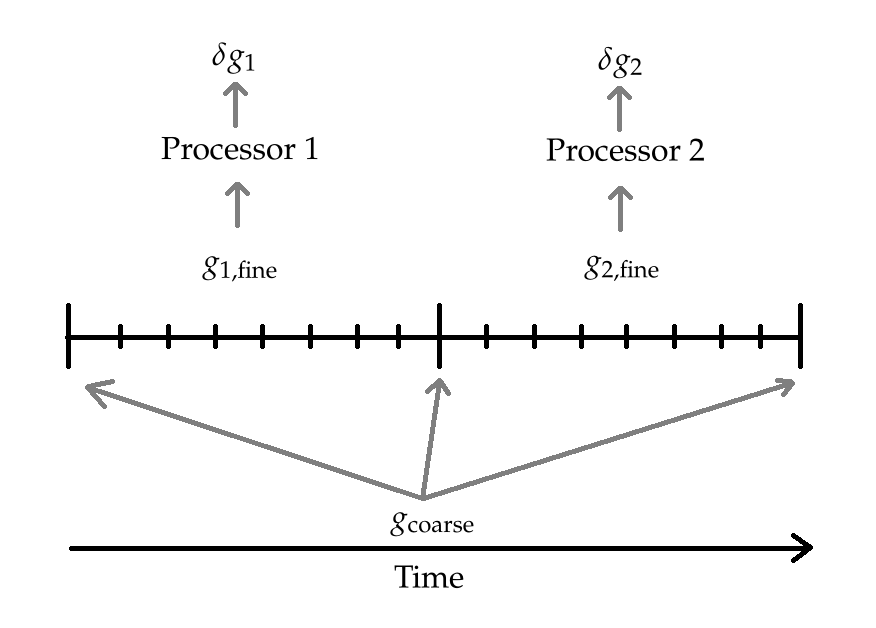
\includegraphics[width=0.75\linewidth]{parareal_visualization.png}
\caption{Graphical representation of the parareal scheme.}
\label{fig:pararealvis}
\end{center}
\end{figure}

\subsection{Convergence of the Parareal}

Assume the coarse operator $g_{\Delta t}$ is Lipschitz and order $m$: for some
constant $L$, 
\[ |g_{\Delta t}(t_n, u) - g_{\Delta t}(t_n, v)| \leq (1 + L \Delta t) |u - v|
\, \forall t \in (0, t_n), \]
\[ |u(t_n) - u^1_N | \leq C(\Delta t)^m |u_0|. \]

Additionally, assume the function $u$ is bounded on $(0, t_n)$. Furthermore,
assume the fine solution operator $g_{\textnormal{fine}}$ is a sufficiently
accurate approximation to the analytic operator so we may replace
$g_{\textnormal{fine}} \to g$. 

\textbf{Theorem}: The order of accuracy of the Parareal method with coarse
solution operator $g_{\Delta t}$ and fine operator $g$ is $mk$. We can prove
this using induction~\cite{bal2005convergence}. 

\emph{Proof}: By induction. 

Case $k = 1$: This is just the coarse operator, which is order $m$. 

Assume that this is true for $k$, that $|u(t_N) - u^k_N| \leq C(\Delta t)^{mk}
|u_0|$. 

For the case $k + 1$, we have
\[
\begin{aligned}
    |u(t_N) - u^{k+1}_N| &= 
    |g(u(t_{N-1})) - g_{\Delta t}(u^{k+1}_{N-1}) - \delta g(u^k_{N-1})| \\
    &= |g_{\Delta t}(u(t_{N-1})) - g_{\Delta t}(u^{k+1}_{N-1}) - \delta
    g(u^k_{N-1}) + \delta g(u(t_{N-1}))| \\
    &\leq |g_{\Delta t}(u(t_{N-1})) - g_{\Delta t}(u^{k+1}_{N-1})| - |\delta
    g(u^k_{N-1}) + \delta g(u(t_{N-1}))| \\
    &\leq (1 + C \Delta t) |u(t_{N-1} - u_{N-1}^{k+1}| + C(\Delta t)^{m+1} |
    u_{N-1}^k - u(t_{N-1}) | \\
    &\leq (1 + C \Delta t) |u(t_{N-1}) - u_{N-1}^{k+1}| + C(\Delta t)^{m(k+1)+1}
    | u_0 | \\
\end{aligned}
\]

We can continue to expand $|u(t_{N-1} - u_{N-1}^{k+1}|$ and get time indices of
$N-1, N-2, \ldots, 2, 1$. This implies that 
\[ |u(t_N) - u^{k+1}_N| \leq C(\Delta t)^{m(k+1)} |u_0|, \]
as desired. 

\subsection{Error of the Parareal}

With the assumptions of the previous section, this parareal method will
approach, with large enough $k$ (correction iterations) to approach the error of
the fine method. However, there is a time vs. accuracy tradeoff. Let $Q$ be the
\emph{Quality Factor} for $g_{\Delta t}$ and $g_{\textnormal{fine}}$. Suppose
that, for constant number of processors and $\Delta t$, $g_{\Delta t}$ runs in
time $T$. Then, $g_{\textnormal{fine}}$ runs in time $QT$. With too large of a
$k$ and a lower $Q$, the time for the Parareal could potentially take longer
than the direct serial computation. We note that there could be other
relationships between the time of the coarse and fine schemes other than
multiplication by a constant term. 

Disregarding the time relationship between $g_{\Delta t}$ and
$g_{\textnormal{fine}}$, we can look at what happens to the error as $k \to N$
(recall that $N$ is the total number of time points in the time discretization). 

For $k = 1, 2, \ldots$ we have 
\[u_{n+1}^{k+1} = g_{\Delta t} (t_n, u_n^{k+1}) + \big(
g_{\textnormal{fine}}(t_n, u_n^k) - g_{\Delta t}(t_n, u_n^k)\big). \]

As $k \to N$, the Parareal algorithm gives $u_{n}^{k+1} = u^k_n$, so the order
of accuracy approaches that of $g_{\textnormal{fine}}$. 

\subsection{Stability of the Parareal}

With the Parareal method, it is possible to combine ODE solvers. The stability region depends on both $g_{\Delta t}$ and $g_{\textnormal{fine}}$, and the
equation being solved. 

Let us consider the ODE $du/dt = \lambda u$. Let $g_{\textnormal{fine}}(t_n,
u_n) = \bar{g_{\textnormal{fine}}}u_n$ and $g_{\Delta t}(t_n, u_n) =
\bar{g_{\Delta t}} u_n$. As shown by Staff et al. \cite{staff2005stability}, the parareal method becomes 

\[ u_n^k = \left( \sum_{j=0}^k {n \choose j} (\bar{g_{\textnormal{fine}}} -
g_{\Delta t})^j \bar{g_{\Delta t}}^{n-j} \right) u_0 = H(\bar{g_{\Delta
t}}, \bar{g_{\textnormal{fine}}}, n, k, \lambda)u_0 \]

This is stable if $\textnormal{max}_{n, k} |H| \leq 1$. 

When $\lambda \in \mathbb{R}$ and $\lambda \leq 0$, Staff et. al also show that

\[
    \begin{aligned}
    |H| &\leq \sum_{j=0}^n {n \choose j} |\bar{g_{\textnormal{fine}}} -
    g_{\Delta t}|^j |\bar{g_{\Delta t}}|^{n-j} \\
    &= (|\bar{g_{\textnormal{fine}}} - g_{\Delta t}| + |\bar{g_{\Delta
    t}}|)^n \leq 1
    \end{aligned}
\]

To satisfy these conditions, we have that 
\begin{enumerate}
    \item $| \bar{g_{\textnormal{fine}}} | \leq 1$: This is the usual stability
        requirement.
    \item $|\bar{g_{\textnormal{fine}}} - 2 \bar{g_{\Delta t}}| \leq 1$.
\end{enumerate}


\subsection{Parallel Tradeoff Analysis}

\subsubsection{Parareal}

We look to compute a theoretical maximum speedup enabled by the nature of the Parareal algorithm.  As this is a tradeoff between error (with parameter k being the number of iterations of corrections, each which takes another cycle of $g_{\Delta t}$, we seek to express the tradeoff as a function of the quality factor, $Q$, the number of iterations, $k$ and the number of processors $n$.  Our quality factor is defined as the multiplicative factor of additional time necessary to compute the solution using the $g_{\textnormal{fine}}$ scheme instead of the $g_{\Delta t}$ method.

Then, the runtime of Parareal is, assuming negligible overhead and ignoring communication bandwidth and letting $t$ be the time in seconds to compute the coarse $g_{\Delta t}$:

\begin{equation}
t + k \left(t + \frac{Qt}{N} \right).
\label{eq:scheme}
\end{equation}

The first $t$ seconds comes from the first coarse approximation, without which the parareal algorithm degenerates to $g_{\Delta t}$.  Then for each of the $k$ correction iterations, the $t$ term comes from $n$, element by element evaluations of  $g_{\Delta t}$ followed by a parallel $\frac{1}{N}$ evaluation of $g_{\textnormal{fine}}$. In order for there to be a speedup relative to the fine operator, we can rearrange to get:

\[
\begin{aligned}
t + k\left( t + \frac{Qt}{N} \right) &< Qt \\
k &< \frac{Q - 1}{1 + Q/N} \\
N &> \frac{Qk}{Q - 1 - k} \\
\end{aligned}
\]

This can be tuned with by either adjusting the the quality factor or reducing the number of iterations, but the number of iterations, $k$, is important for error convergence to that of $g_{\textnormal{fine}}$.  However, finding the optimal $k$ is a problem-specific parameter and traded off for the desired accepted error.

\subsubsection{Parallel By Space}

For the parallelism by space, we are dividing our grid on which we which to solve our wave diffusion equation. This division is inherently parallelizable and allows us to follow a very similar approach in computing this as in the serial version - just divided in space, where the stencil approach is well-defined. A fully parallelizable approach allows for $n$ times speedup and no computational tradeoffs if we ignore communication. As we are dividing our processors into a processor grid (dividing a 2D space into a 2D arrangement of processors) we are only limited by when the processor grid size approaches the problem size - upon which further processors would not receive any tasks since that would require a division by less than a unit of computation.

\subsection{Incorporating Communication}

To delve one step deeper in our analysis, parallel communications are usually expressed by architecture parameters - $\alpha$, $\beta$ and $\gamma$ explained in the below table.

\begin{table}
\centering
\begin{tabular}{|c|l|}
{\bf Variable} & {\bf Description}\\
\hline\hline
$\alpha$ & Latency of communication. (sec)\\
$\beta$ & Inverse communication bandwidth. (sec/byte)\\
$\gamma$ & Inverse computational performance. (sec/flop)\\
\hline
\end{tabular}
\caption{Table of Communication Architecture Parameters}
\label{tab:notation}
\end{table}

\subsubsection{Parareal}
TODO THIS IS CONFUSING Wesley


\subsubsection{Parallel By Space}
TODO THIS IS CONFUSING TOO Wesley

\subsection{Amdahl's Law Analysis}

One of the main drawbacks of using Amdahl's Law as benchmarks in analysis is in the generally abstract way the paralleizable fraction is determined, the $B$ term.  The value of this is estimated based on an understanding of the algorithm from a high level and not derived from any underlying mathematical expressions.

\subsubsection{Parareal}

We first try to express $B$ as function of the quality factor $Q$ and the number of correction steps of the parareal $k$.

From our analysis in equation~\ref{eq:scheme}, when we set $N$ to 1 for the generic setup, we see that our total computation is $t + k(t+ Qt)$.  Of this, the only parallelizable part is the $kQt$ term.  Thus to find the expression of the non-parallelizable portion, we simplify:

\[
B = \frac{t+kt}{t+kt+kQt} = \frac{1+k}{kQ+k+1}
\]

Now to replace this into Amdahl's Law, we have:

\[
\begin{aligned}
S(n) &= \frac{T(1)}{T(n)} = \frac{T(1)}{ T(1) \left( B + \frac{1}{n} (1-B) \right)} = \frac{1}{\left( B + \frac{1}{n} (1-B) \right)}\\
       &= \frac{T(1)}{T(1) \left( \frac{1+k}{kQ+k+1} + \frac{1}{n} (1- \frac{1+k}{kQ+k+1}) \right)} \\
       &= \frac{n(kQ+k+1)}{n+nk+kQ}
\end{aligned}
\]

As written below, we have used $Q = 100$ with various $k$.

When $k = 2$ and $Q = 100$, for maximal speedup (fewest iterations) of $S(n) = \frac{203n}{3n+200} \approx 67$

When $k = 10$ and $Q = 100$, for more iterations and less error, we'd see an Amdahl bounded max speedup of $S(n) = \frac{1011n}{11n+1000} \approx 91$

It is important to note that this speedup is measured with respect to the parareal agorithm done in parallel. This does not compare the Parareal to doing $g_{\textnormal{fine}}$ but rather shows how given infinite processors, our speedup will approach certain asymptotic bounds. We do see however large constants in the denominator which means that we will get better speedup as we increase n past a certain size.

\subsubsection{Parallel By Space}

Because this task is embarassingly parallel and nearly 100% of the computation code can be parallelized (disregarding any uneven divisions of the space by the number of processors), we achieve the Amdahl's Law optimal speedup bound of (with $B$ of 0):

\[
S(n) = \frac{T(1)}{T(n)} = \frac{T(1)}{ T(1) \left( B + \frac{1}{n} (1-B) \right)} = \frac{T(1)}{T(1) \left( 0 + \frac{1}{n} (1-0) \right)} = \frac{T(1)}{T(1) * \left( \frac{1}{n} \right) } = n
\]

With embarassingly parallel problem setups, we can optimally achieve up to $n$ times speedup with $n$ processors though this number if quite ideal and will be very difficult to approach (large scaling will have different memory management and greater communication overheads and costs).

\subsection{Planned Tests to Run}

We wished to explore certain tests that would demonstrate the effects of changing various parameters be it from the solution schemes in the parareal to the exact system we were trying to solve.

Due to the sheer number of things to explore, we usually try to compare each run to a benchmark we decided was most useful for comparison's sake and the list of parameters we wished to test are:

\begin{itemize}
\item General Scaling with Incrased $N$
\item Adjusting $K$ in the Parareal
\item Using Different Integration Schemes in Parareal for $g_{\textnormal{fine}}$
\item Run the Solver on Various Complexities of ODEs
\end{itemize}

\section{Results and Discussion}

WESLEY ENDED HERE, BEFORE THIS IS WESLEY APPROVED

\subsection{Expectations}
We hoped to show that under the properly tuned parameters (namely the $k$ number of iterations),

\subsection{General Remarks about Results}
LETS SEE IF I HAVE TO DISCLAIM ANY GLOBAL FAILURES IN OUR RESULTS

\subsection{Comparison to Serial with $g_{\textnormal{fine}}$ as a Forward Euler with
Smaller $\Delta t$}

We implemented the Parareal algorithm in Python, using mpi4py to parallelize it.
Our coarse operator was forward Euler step, with 100 steps, while the fine
operator was forward Euler, with $Q \cdot 100$ steps, where $Q$ is the quality
factor. We tested the Parareal algorithm on two sets of differential equations:

\[
y'(t) = f(t, y) = \lambda y, \, \, y(0) = 1
\]
\[
y''(t) + 2y'(t) + 5y(t) = 0, \, \, y(0) = 1, \, y'(0) = 0.
\]

We ran the algorithm on different numbers of processors and varied $k$ and $Q$. 

Varying Iterations:

Varying Quality Factor:
We define the quality factor in this case for how many times smaller the Euler method used for $g_{\textnormal{fine}}$ is compared to the Euler method used for $g_{\Delta t}$

Changing the ODE

TODO ashi sort out the figure and match and replace if needbe

\begin{figure}
\begin{center}
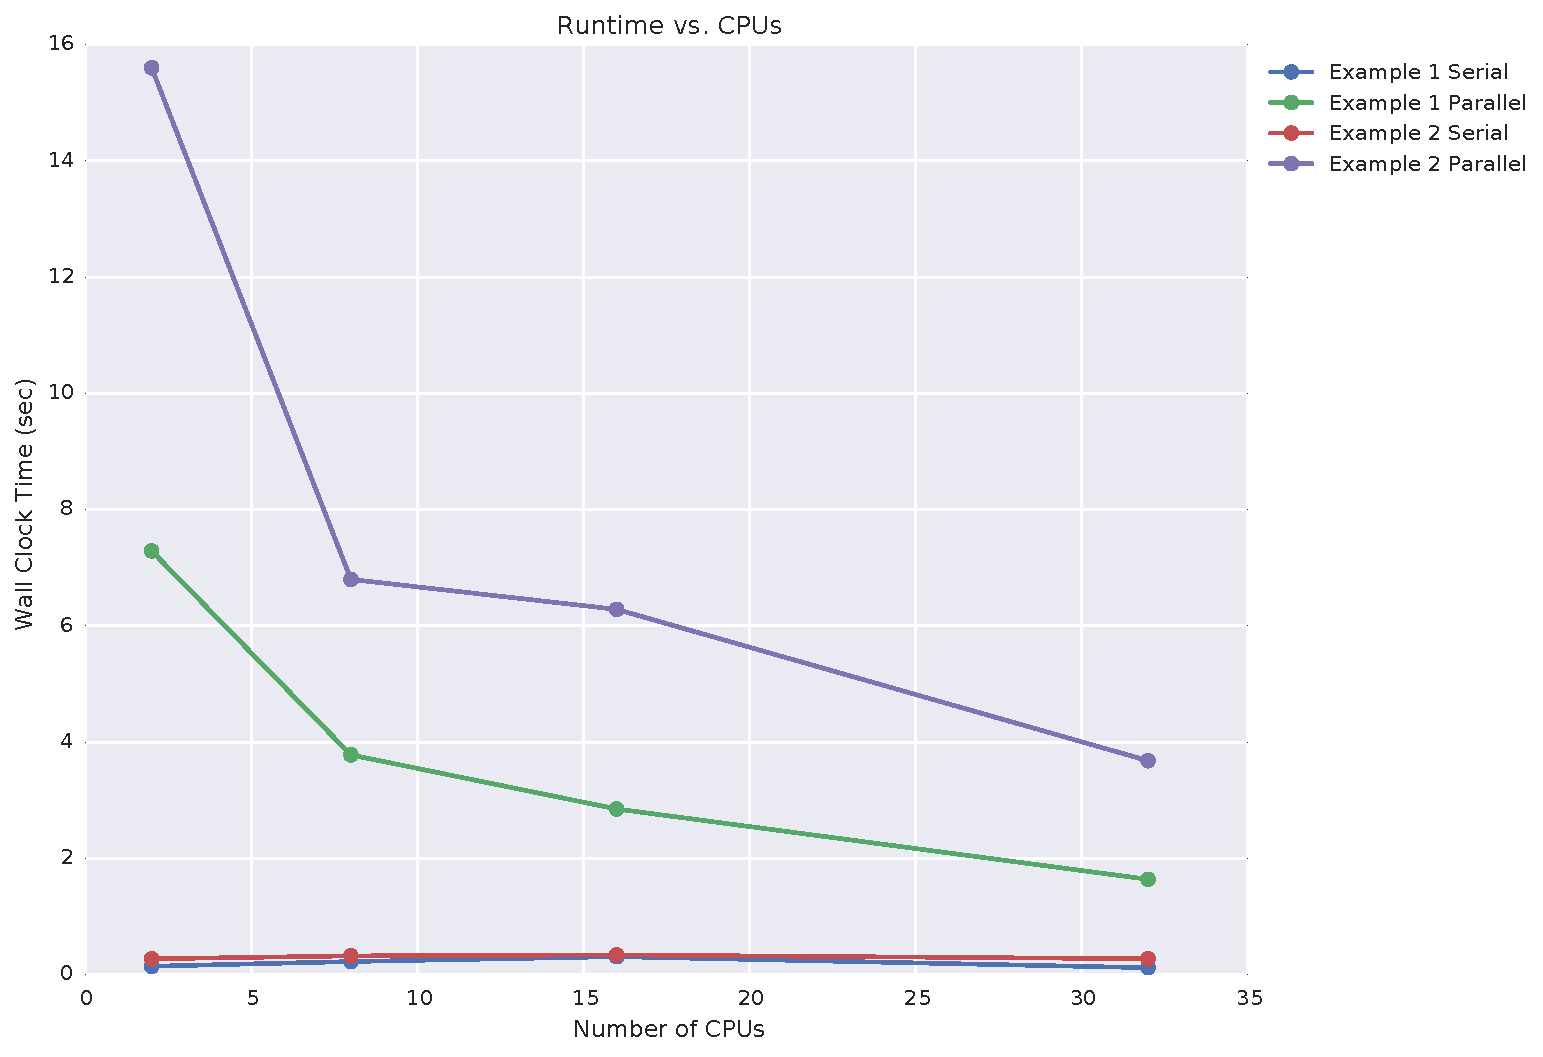
\includegraphics[width=0.75\textwidth]{data/runtime_vs_cpus.pdf}
\caption{Running time vs. number of CPUs.}
\label{fig:run_v_cpu}
\end{center}
\end{figure}

\begin{figure}
\begin{center}
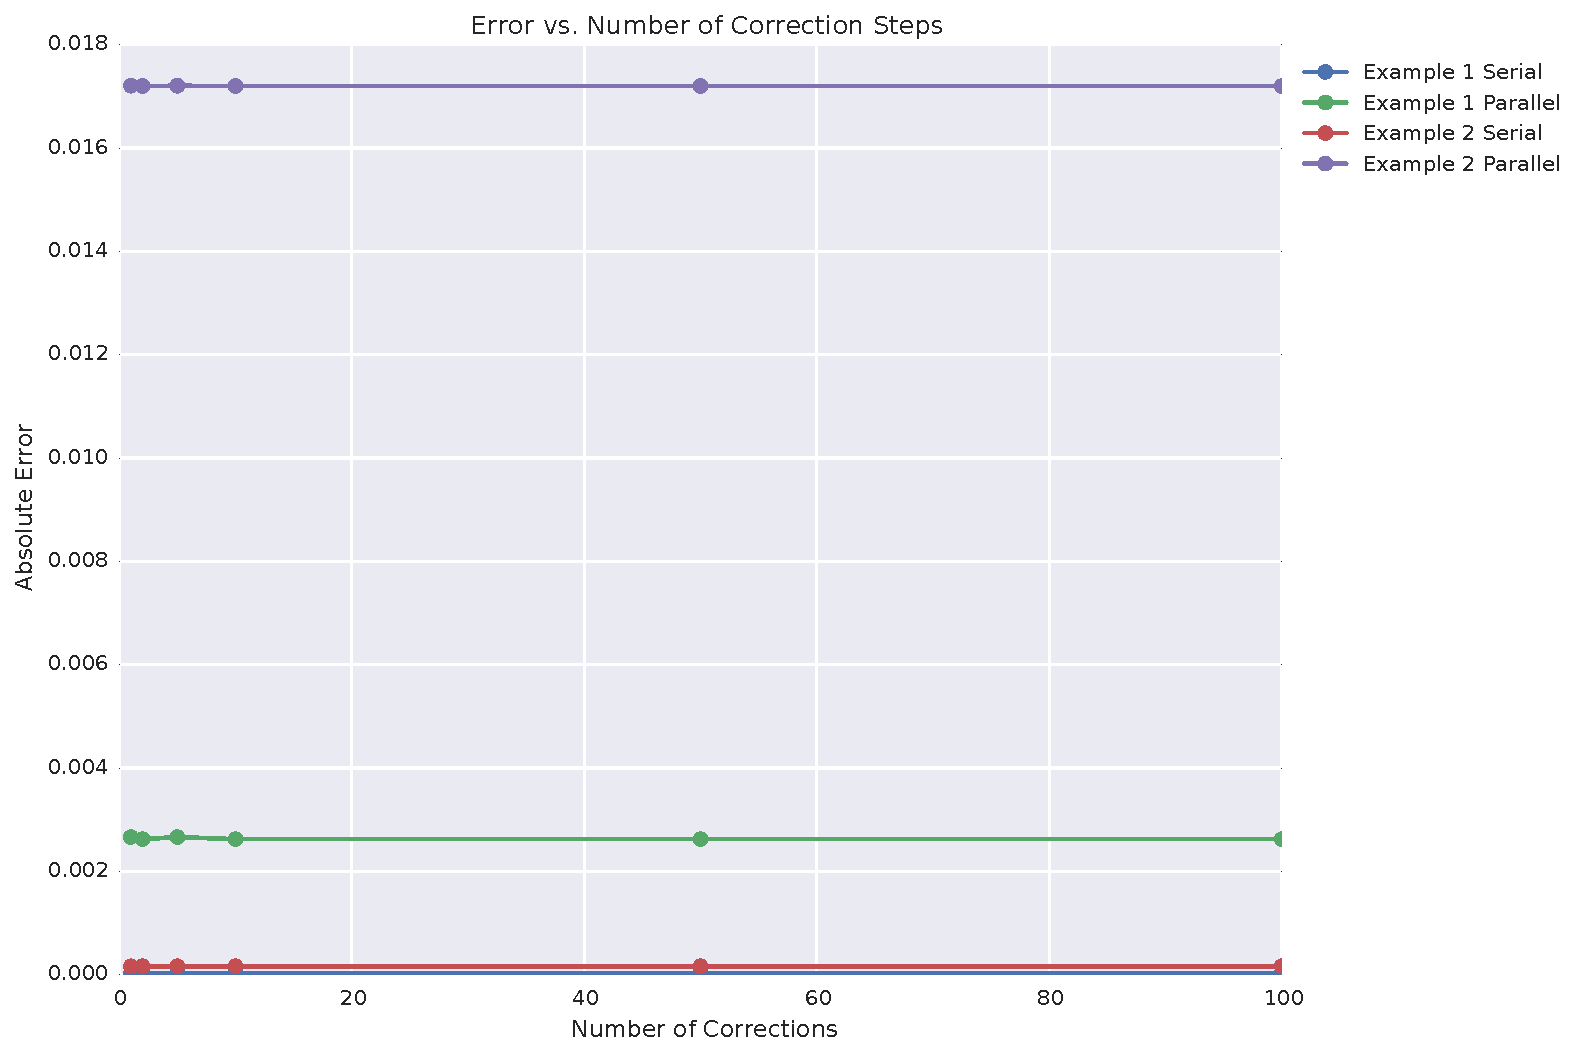
\includegraphics[width=0.75\linewidth]{data/error_vs_corrections.pdf}
\caption{Error vs. number of correction steps.}
\label{fig:err_v_k}
\end{center}
\end{figure}

\begin{figure}
\begin{center}
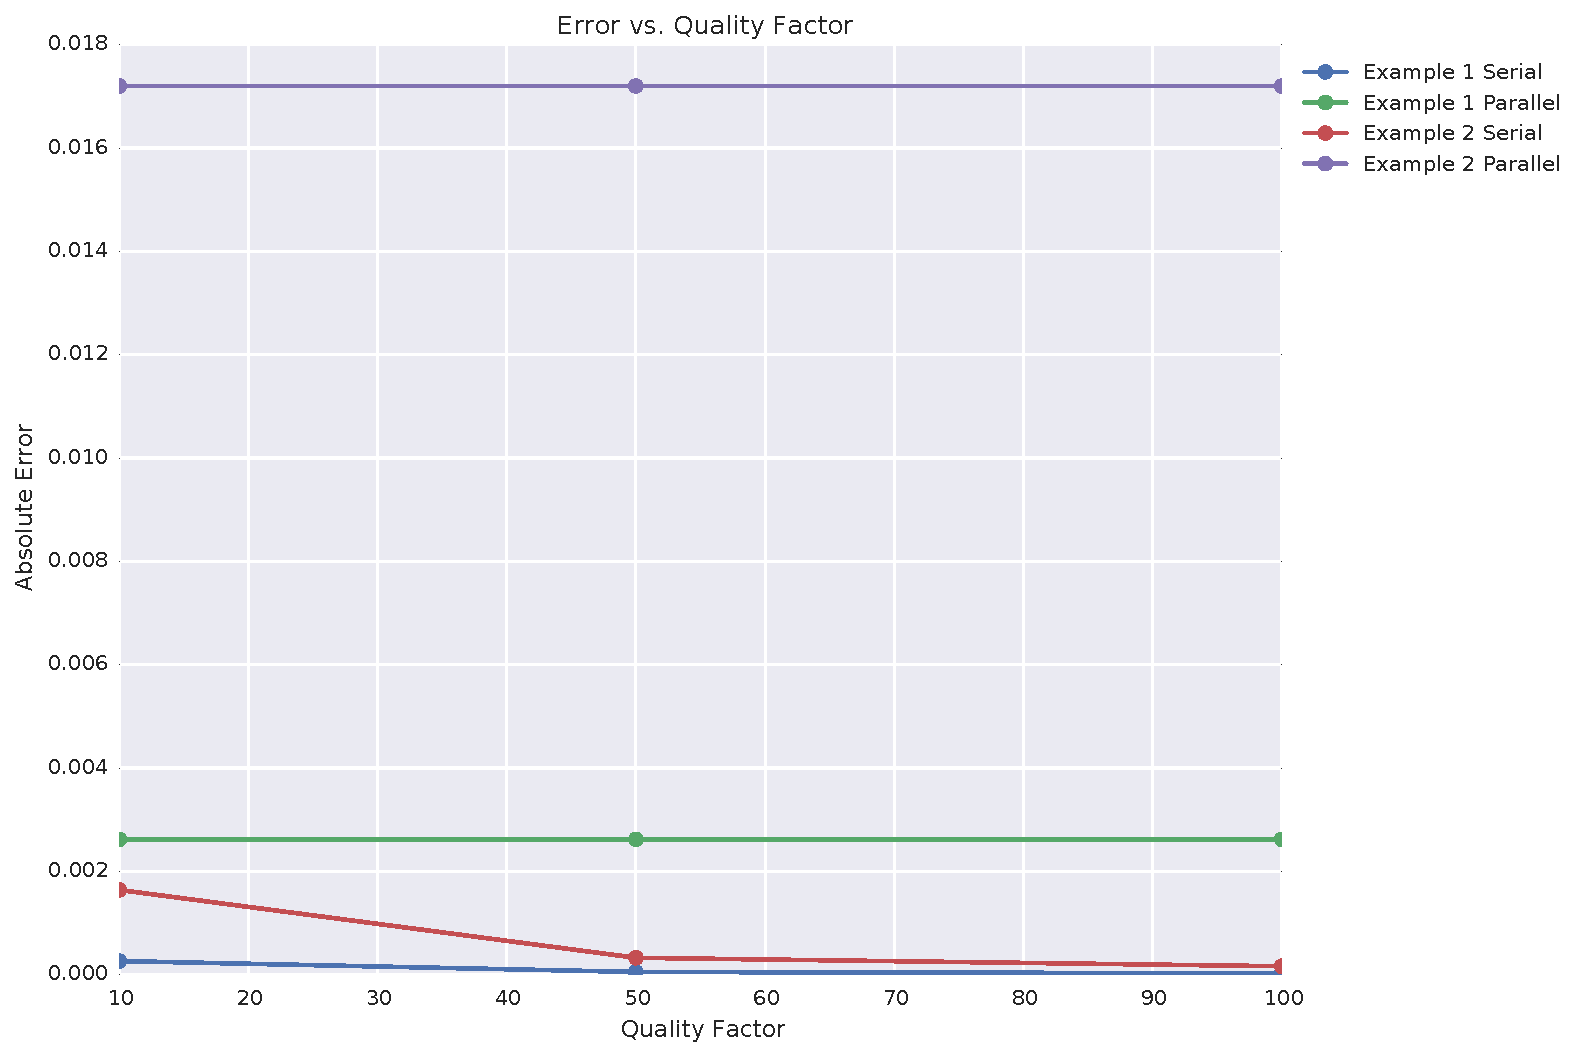
\includegraphics[width=0.75\linewidth]{data/error_vs_qualityfactor.pdf}
\caption{Error vs. quality factor of the fine operator}
\label{fig:err_v_q}
\end{center}
\end{figure}

\begin{figure}
\begin{center}
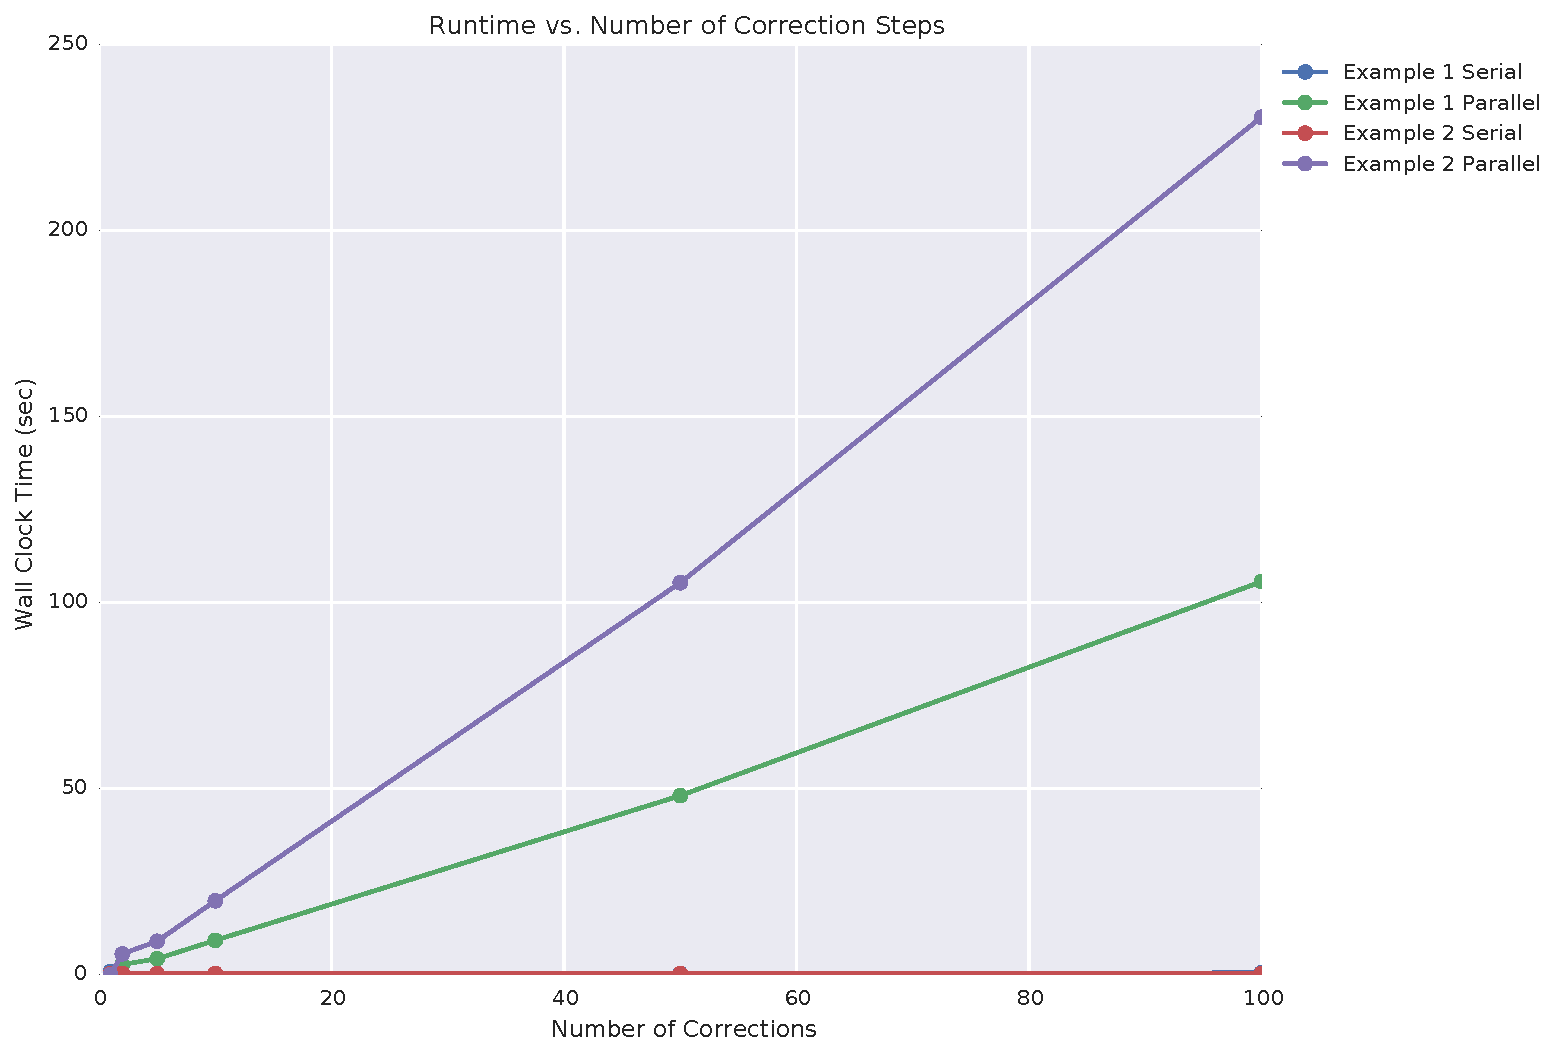
\includegraphics[width=0.75\linewidth]{data/runtime_vs_corrections.pdf}
\caption{Running time as a function of the number of correction steps.}
\label{fig:run_v_k}
\end{center}
\end{figure}

\subsection{Comparison to Serial with $g_{\textnormal{fine}}$ as Higher Order Methods}

TODO team

IDEALLY WE SHOW THE SAME GRAPHS AS THE ABOVE WITH ALL THE VARIATIONS TESTED

\subsection{Parallelism by Space Paradigm}

To demonstrate parallelism by space, we solve the two-dimensional wave equation by partioning a two-dimensional space domain amongst multiple processors. Specifically, we look to numerically solve

\begin{equation*}
\frac{\partial^2 u}{\partial t^2} = \frac{\partial^2 u}{\partial x^2} + \frac{\partial^2 u}{\partial y^2}
\end{equation*}

on the two-dimensional domain $(x, y) \in [0,1]\times[0,1]$ for evolution in time. We partition the domain by space using a second order central difference approximation, assigning a rectangular portion of the two-dimensional domain to each of a grid of $(P_x, P_y)$ processors. This requires the passing of information along the edges of the processors to each other, as shown graphically in the figure below:

\begin{figure}[H]
\begin{center}
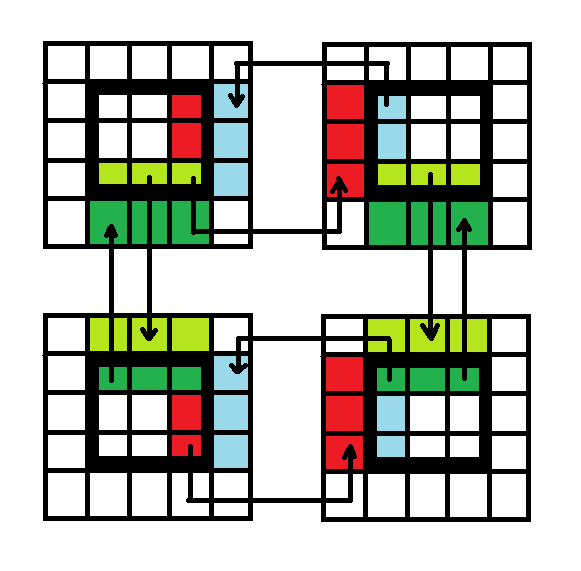
\includegraphics[width=0.5\linewidth]{decomp.png}
\caption{Parallelization by space schematic.}
\label{fig:spaceparallel}
\end{center}
\end{figure}

Note that each processor receives information from only those adjacent to it; that is, the top left processor in the graphic does not communicate directly with the bottom right processor in the graphic. Rather, information is passed only along shared boundary points to propagate the wave equation. We run this code for three different grid sizes: $128\times 128$, $256\times 256$, and $512\times 512$, in both serial and parallel.

In serial, we have:

\begin{center}
\begin{tabular}{|c|c|} \hline
($N_x, N_y$) & Time (seconds)\\ \hline
(128, 128) & 0.987\\ \hline
(256, 256) & 7.889\\ \hline %real
(512, 512) & 63.913\\ \hline %real
\end{tabular}
\end{center}

In parallel, we have:

\begin{center}
\begin{tabular}{|c|c|c|c|c|} \hline
($N_x, N_y$) & $P_x$ & $P_y$ & Time (sec) \\ \hline
(128, 128) & 2 & 2 & (still queued on Odyssey)\\ \hline
(128, 128) & 4 & 2 & 2.31 \\ \hline
(128, 128) & 4 & 4 & (still queued on Odyssey) \\ \hline
(128, 128) & 8 & 8 & (still queued on Odyssey) \\ \hline
(256, 256) & 2 & 2 & 2.57 \\ \hline %real
(256, 256) & 4 & 2 & 11.32 \\ \hline
(256, 256) & 4 & 4 & 13.65 \\ \hline
(256, 256) & 8 & 8 & 17.44 \\ \hline
(512, 512) & 2 & 2 & (still queued on Odyssey)\\ \hline
(512, 512) & 4 & 2 & (still queued on Odyssey)\\ \hline
(512, 512) & 4 & 4 & (still queued on Odyssey)\\ \hline %check
(512, 512) & 8 & 8 & (still queued on Odyssey) \\ \hline %check
\end{tabular}
\end{center}

Note that as the workload assigned to each processing element stays constant and more processors are used to solve a larger problem, near-linear scaling is achieved. However, scaling is \textbf{not} achieved when we simply add more processing elements to try to solve the same-sized problem, as there is greater constant startup costs which do not necessarily improve the speed (or perhaps even decrease speed). Hence, this is an example of weak scaling. However, an advantage to this paradigm is that because each processor only communicates with its nearest neighbors, communication overhead is relatively constant regardless of how large problem size / number of processors used becomes. Therefore, such a paradigm should scale well to larger problem sizes or more fine grid spacings. 


\subsection{Summary of Performance}

TODO team

\subsection{Demonstrating Scaling and Efficiency}

\subsection{Parallel in Space}

bsim TODO eventually

As we can see, we do see the effects of WEAK scaling

TODO analyze

\subsection{Possible Optimizations and Future Work}

We see that (HOPE IT WORKS WELL OR ELSE...) Most of the further work would be in
optimization. We are trying to measure performance in Python, which is not the
ideal benchmarking language for efficiency and speedups. A port over to C++
using the MPI libraries in C++ rather than the mpi4py libraries in python would
be ideal. Other optimizations mentioned above could also be implemented. To
further explore the parareal algorithm would involve many test cases and to see
how the parareal algorithm compares to other approaches---since the actual time
and iterations necessary depend on the system of ODEs to solve.


TODO NUMPY WRITE FATST HING

On the other hand, parallelism by space already requires a more problem-specific
design. Parallelism by space is intuitive, and conceptually, is embarrassingly parallel and easier to create. However, the
limitations are in the requirement for the code to be designed for the
problem---how to divide by space so as to allow for the maximum number of even
divisions. The lack of generality is not as beautiful as the parareal algorithm
but may lend itself to faster speedups.

TODO WRITE ABOUT BETTER DATA COLLECTION

\section{Conclusion and Future Work}

All in all, we have implemented and begun to explore some techniques of looking
for strong and weak scaling efficiencies for solving ODEs. The parareal
algorithm is beautiful in its theoretical advantages---in terms of stability,
error and efficiency. However, the method, as a very generalized method,
requires deeper analysis for the specific problem. The main variable will be in
the difference in the coarse and fine methods (be it lower and higher order or a
higher and lower resolution for the same method). The tradeoffs that must be
computed and optimized for would be problem specific.

\nocite{*}
\bibliographystyle{unsrt}
\bibliography{paper}

Bibtex Citations for the Slides, and for \url{https://www.sharcnet.ca/help/index.php/Measuring_Parallel_Scaling_Performance}

\end{document}
